%===================================================================================
% PREÁMBULO
%-----------------------------------------------------------------------------------
\documentclass[a4paper,10pt,twocolumn]{article}

%===================================================================================
% Paquetes
%-----------------------------------------------------------------------------------
\usepackage{amsmath}
\usepackage{amsfonts}
\usepackage{amssymb}
\usepackage{informe}
\usepackage{lipsum}
\usepackage[utf8]{inputenc}
\usepackage{listings}
\usepackage{algorithmic}
\usepackage[pdftex]{hyperref}
%-----------------------------------------------------------------------------------
% Configuración
%-----------------------------------------------------------------------------------
\hypersetup{colorlinks,%
	    citecolor=black,%
	    filecolor=black,%
	    linkcolor=black,%
	    urlcolor=blue}

%===================================================================================



%===================================================================================
% Presentacion
%-----------------------------------------------------------------------------------
% Título
%-----------------------------------------------------------------------------------
\title{Proyecto de Estad\'istica \\ 2da Fase}

%-----------------------------------------------------------------------------------
% Autores
%-----------------------------------------------------------------------------------
\author{\\
	\name Eric Martin Garcia \\ \addr Grupo C411 \\
	\name Carlos Rafael Ortega Lezcano \\ \addr Grupo C411 \\
	\name Harold Rosales Hernandez \\ \addr Grupo C411 }


%-----------------------------------------------------------------------------------
% Tutores
%-----------------------------------------------------------------------------------
\tutors{\\}

%-----------------------------------------------------------------------------------
% Headings
%-----------------------------------------------------------------------------------
%\jcematcomheading{\the\year}{1-\pageref{end}}{Carlos Rafael}

%-----------------------------------------------------------------------------------
%\ShortHeadings{Simulacio\'n basada en Eventos Discretos}{Carlos Rafael}
%===================================================================================



%===================================================================================
% DOCUMENTO
%-----------------------------------------------------------------------------------
\begin{document}

%-----------------------------------------------------------------------------------
% NO BORRAR ESTA LINEA!
%-----------------------------------------------------------------------------------
\twocolumn[
%-----------------------------------------------------------------------------------

\maketitle

%===================================================================================
% Resumen y Abstract
%-----------------------------------------------------------------------------------
\selectlanguage{spanish} % Para producir el documento en Español

%-----------------------------------------------------------------------------------
% Palabras clave
%-----------------------------------------------------------------------------------
%\begin{keywords}
%	Separadas,
%	Por,
%	Comas.
%\end{keywords}

%-----------------------------------------------------------------------------------
% Temas
%-----------------------------------------------------------------------------------
%\begin{topics}
%	Tema, Subtema.
%\end{topics}


%-----------------------------------------------------------------------------------
% NO BORRAR ESTAS LINEAS!
%-----------------------------------------------------------------------------------
\vspace{0.8cm}
]
%-----------------------------------------------------------------------------------


%===================================================================================

%===================================================================================
% Introducción
%-----------------------------------------------------------------------------------
\section*{Introducción}\label{sec:intro}
%-----------------------------------------------------------------------------------
En este trabajo se realizará un estudio de los datos de los jugadores del FIFA19 usando las técnicas de regresión, reducción de dimensión y de ANOVA.

\begin{enumerate}
	\item Se elegirán las variables a las se cuales les aplicara cada técnica y se explicará el por qué.
	\item En las técnicas que lo requieran,  se realizará el análisis de los supuestos y se explicará si es válida la aplicación de la técnica en esa variable.
\end{enumerate}


\section*{Desarrollo}\label{sec:dev}
  
\subsection*{Regresión Múltiple}

En este apartado se trabajará sobre el subconjunto de jugadores de campo del FIFA19 que pertenecen al club Inter de Milán.
En primer lugar se analiza la relación entre las variables utilizando la matriz de correlación "\verb|cor(dataset)|", resultando:

\begin{figure}[h]
	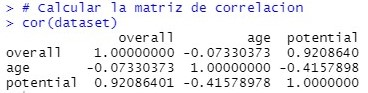
\includegraphics[scale=0.86]{./imgs/reg_correlation.jpg}
\end{figure}

El modelo elegido buscará analizar la relación de la variable (\textit{overall}) con las variables (\textit{age}) y (\textit{potential}), quedando representado de la siguiente forma:

\begin{align*}
overall = \beta_0 + potential \beta_1 + age \beta_2 + e
\end{align*}

Para investigar los resultados de la regresión y determinar el valor de los $\beta_j$ se utilizó la función "\verb|summary(regression_model)|" de \verb|R| y se obtuvo la salida mostrada en la Figura 1\\\\\\

\begin{figure}[h]
	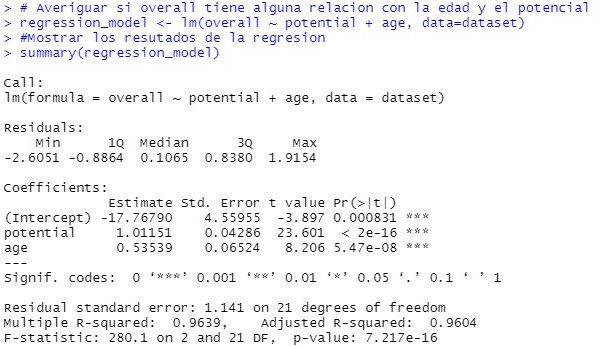
\includegraphics[scale=0.7]{./imgs/reg_model.jpg}
\end{figure}

Sustituyendo los valores obtenidos resulta el modelo:

\begin{align*}
\widehat{overall} = 1.01151 potential + 0.53539 age - 17.76790
\end{align*}

\textbf{Coeficientes}: Los coeficientes son significativos al $0\%$ inclusive el intercepto lo que es bueno para el modelo, los valores de $Pr(>|t|)$ son menores que 0.05 por lo tanto todas las variables aportan información al modelo.\\

\textbf{Adjusted R-Square}: El valor del R-Cuadrado es 0.9604 por lo tanto el modelo se considera muy bueno en cuanto a la realizaci\'on de predicciones\\

\textbf{F-Statistic}: Su valor menor que 0.05 nos indica la existencia de al menos una variable que esta siendo significativa para el modelo

\newpage

\textbf{Analizando los Residuos}:

\begin{enumerate}
	\item[1.] \textbf{La media de los errores es 0 y la suma de los errores es 0}:

\begin{figure}[h]
	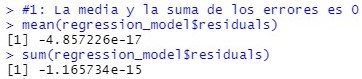
\includegraphics[scale=0.8]{./imgs/reg_1.jpg}
\end{figure}
	
	\item[2.] \textbf{Errores normalmente distribuidos}:\\
	Se muestra el histograma y el Normal Q-Q Plot ,en el histograma se puede apreciar un parecido a una distribuci\'on normal y al observar el QQ Plot se aprecia como la mayoría de los puntos de residuo se encuentran sobre la recta, por lo tanto se asume una normalidad en los errores del modelo (\textbf{Figura 2})
	
	\begin{figure}[h]
		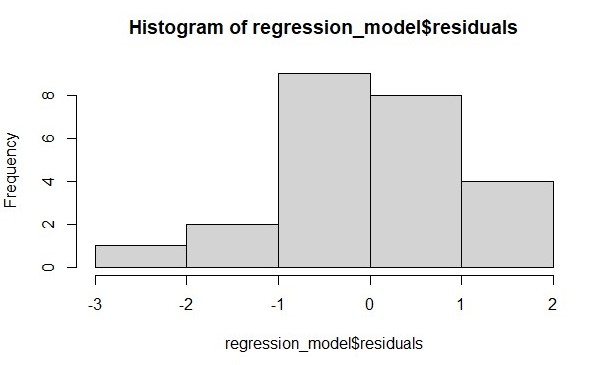
\includegraphics[scale=0.5]{./imgs/reg_2_hist.jpg}
		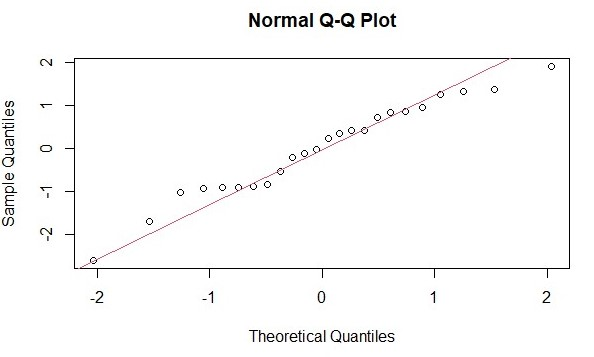
\includegraphics[scale=0.5]{./imgs/reg_2_qq.jpg}
		\caption{}
	\end{figure}
	
	\item [3.] \textbf{Independencia de los residuos}:\\
	Para la prueba de independencia se emplea la prueba Durbin-Watson:
	
	\begin{figure}[h]
		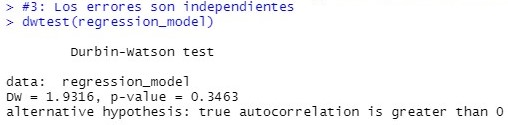
\includegraphics[width=0.5\textwidth]{./imgs/reg_3.jpg}
	\end{figure}
	
	Como el p-value es mayor que 0.05 no se puede rechazar la hipótesis nula, por lo tanto se puede afirmar que los errores son independientes. \\
	
	\item[4.] \textbf{La varianza de los errores es constante (Homocedasticidad)}:\\
	
	Se puede observar en el gráfico el cumplimiento de la homocedasticidad:
	
	\begin{figure}[h]
		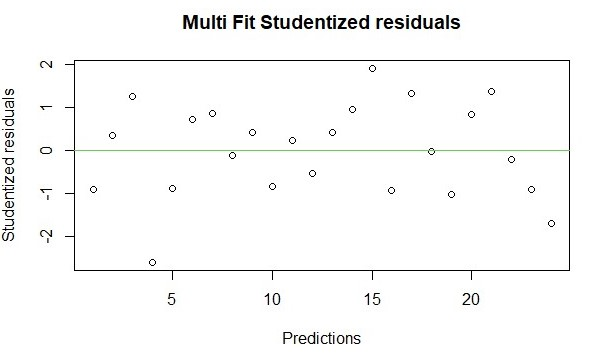
\includegraphics[scale=0.4]{./imgs/reg_4.jpg}
	\end{figure}
	
\end{enumerate}


\subsection*{ACP}

En este apartado se trabajará sobre el subconjunto de jugadores de campo del FIFA19 que pertenecen al club FC Barcelona.\\
En primera instancia se hace un análisis de la correlación en la muestra utilizando la matriz de correlación  "\verb|cor(acp_dataset)|" y la función "\verb|symnum(tp)|" presente en \verb|R|, que retorna de forma gráfica si dicha matriz esta o no, altamente correlacionada, resultando:

\begin{figure}[h]
	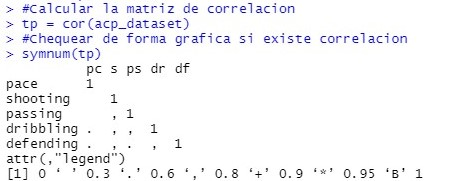
\includegraphics[scale=0.7]{./imgs/acp_correlation.jpg}
\end{figure}

Se puede observar que no existe una relación entre las variables por lo tanto se procede a reducir dimensión. Para esto se seleccionan las componentes principales:

\begin{figure}[h]
	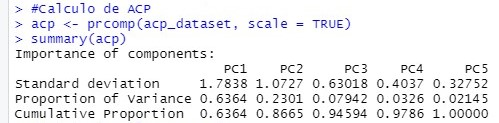
\includegraphics[scale=0.6]{./imgs/acp_summary.jpg}
\end{figure}

Para la selección de las componentes principales se procede a graficar los valores propios asociados a cada una ellas:

\begin{figure}[h]
	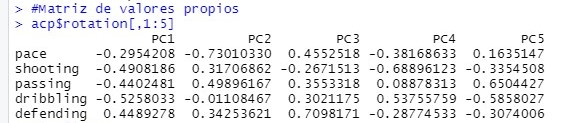
\includegraphics[scale=0.1]{./imgs/acp_vp.jpg}
\end{figure}


Para la selecci\'on de las componentes principales empleamos la proporci\'on acumulativa y nos quedamos con aquellas que su porciento acumulatico es menor que 0.70 y la primera que supera este valor, seg\'un lo visto en el criterio del porcentaje, adem\'as si observamos detenidamente los valores propios las tres primeras componentes tienen valor propio mayor a 1 por tanto si hubieramos seleccionado el criterio de Kaiser obtendriamos las 3 primeras componentes como principales.\\
Los valores propios de las 3 primeras componentes son los siguientes:

\begin{figure}[h]
	\includegraphics[scale=0.5]{./imgs/main.png}
\end{figure}


Ahora pasemos a analizar cuales variables son importantes en cada componente y en que medida, para esto tomamos por cada componente el mayor valor propio $\lambda_i$, dividimos entre 2 y todo valor propio cuyo valor absoluto este por encima de $\lambda_i / 2$, la variable asociada a este conformar\'a la componente.

\begin{enumerate}
	\item[] \textbf{PC1} ($\lambda_{\max} = 0.61$): Esta componente esta caraterizada por una muestra de jugadores de bajo \textit{overall}, con poco desarrollo en el juego (\textit{potential}) y de baja reputaci\'on internacional, o sea no ser\'an convocados a la selecci\'on con mucha frecuencia
	
	\item[] \textbf{PC2} ($\lambda_{\max} = 0.65$): Esta componente esta caracterizada por una muestra de
	jugadores j\'ovenes con buenas habilidades en el dominio del bal\'on, adem\'as el valor negativo en la variable altura puede asociarse a jugadores del mediocampo, en su mayoria en lugar de defensores y delanteros centros
	
	\item[] \textbf{PC3} ($\lambda_{\max} = 0.72$): Esta componente esta caracteriza por una muestra de 
	jugadores j\'ovenes con gran potencial (a medida que avancen las temporadas su promedio y valor aumentar\'a en gran medida). Esta componente resulta interesante porque describe a aquellos jugadores que podr\'iamos elegir en el juego para el pasar las temporadas sea de gran valor para nuestro equipo 
\end{enumerate} 

La figura siguiente muesta los biplot para las 2 primeras componentes (PC1, PC2) y para las dos \'ultimas (PC2, PC3):

\begin{figure}[h]
	\verb|> biplot(acp, choices = 1:2)|
	
	\includegraphics[scale=0.4]{./imgs/biplotp1p2.jpeg}
	\verb|> biplot(acp, choices = 2:3)|
	
	\includegraphics[scale=0.4]{./imgs/biplotp2p3.jpeg}
\end{figure}

\section*{Conclussion}\label{sec:con}

\lipsum[9-11]

\begin{thebibliography}{9}
	
\end{thebibliography}

\label{end}

\end{document}

%===================================================================================
